\section{Grid-search on DNN parameters}
\label{sec:gridsearches}

\paragraph{\textbf{Grid-search on optimizer, activation functions and dropout probabilities -}}
We have picked several candidates for these three parameters in order to test their combinations using a huge initial grid-search. We tested 200 epochs for each combination, using a 4-fold cross validation.

From this grid-search we got many combinations which achieved an almost perfect accuracy ($\sim 99\%$), while there exists some combinations which lead to very bad accuracy ($\sim 50\%$, i.e. a random guess). In the poll of the best classifiers (see the output in the attached Jupyter notebook), we see that \emph{Nadam}, \emph{Adam} and \emph{RMSprop} optimizers, combined with \emph{softplus}, \emph{softsign} and \emph{tanh} activation functions typically lead to better results. Also, lower dropout values are very common among the best classifiers. From now on we restrict the DNN model to the previously listed parameters, as well as the small dropout values from $0.0$ (no dropout) up to $0.3$.


\paragraph{\textbf{Grid-search on layer configuration - }} We want to probe the impact on the accuracy due to the number of neurons in the layers, as well as to the number of layers itself. Therefore, in this second grid-search we will test DNNs with $q = [1,2,3,4,5,6]$ layers in grid-combination with $s = [10,20,30,40,50]$ neurons per layer. The general rule is that each DNN will have a certain amount $q$ of layers, all of same size $s$. Explicitly, a first DNN might have two layers of 30 neurons each; another one might have three layers of 50 neurons each. All the possible DNNs are also tested by varying the hyper-parameters selected in the first grid search.

Instead of looking at the spurious results of this grid-search, it is interesting to notice how the accuracy declines when we reduce the number of layers. Indeed, it is trivial that deeper DNN will more likely achieve better results. Figure \ref{fig:layer_performances} shows that 1-layer DNNs are more likely to achieve an accuracy $\sim 90\%$, while 2-layer DNNs do slightly better $\sim 95\%$. The DNNs with 3 and more layers are more likely to saturate the accuracy $\sim 99\%$.

\begin{figure}[h]
  \centering
  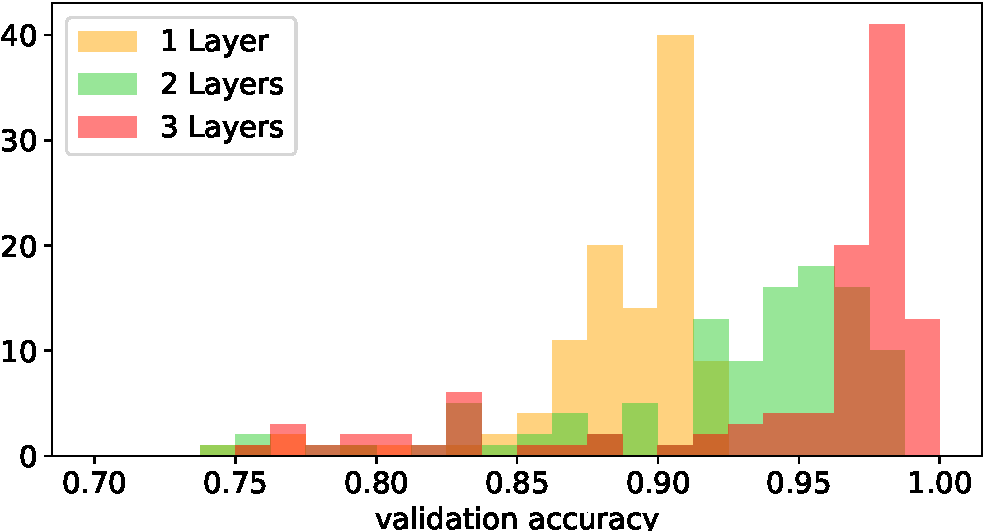
\includegraphics[width=\columnwidth]{hist_layers_1_crop.pdf}
  \caption{The accuracy distribution based on the layer configuration grid-search. } %The histogram shows how the average performance of the models declines when the number of layers is further reduced.
  \label{fig:layer_performances}
\end{figure}

%It is important to note that the worst score in this last test is 0.967813, meaning that the restrictions that were imposed to the Activations, Dropout and Optimizer parameters secure a high performance of the Neural Network. While trying different combinations of Layers and Layer Size just varied the score from in a range of +/- 1.1718\%, showing that the impact of conducting a gridsearch with many variations of this parameters is minimal compared to the previous three.